\documentclass[a4paper]{article}

\usepackage[english]{babel}
\usepackage[utf8x]{inputenc}
\usepackage{amsmath}
\usepackage{graphicx}
\usepackage[colorinlistoftodos]{todonotes}
\usepackage{listings}
\usepackage[export]{adjustbox}

\title{Organisation in Twitch Plays Pokemon}
\author{Léonard Allain-Launay}

\begin{document}
\maketitle

\begin{abstract}
A hundred thousand players playing simultaneously the same game succeeded in finishing \textit{Pokemon : Red} in sixteen days. How did they manage that ?
\end{abstract}

\section{Twitch Plays Pokemon}
\textit{Twitch Plays Pokemon} (\textit{TPP}) is a collaborative game that started on the Twitch platform on February 12th 2014. It was also described first by its creator as a \textit{social experiment}, to see what would happen if an unlimited number of people were playing the same player in a video game at the same time. \textit{Twitch} is a web platform allowing video gamers to broadcast their games to the public, to show off their skills, explain strategies, stream e-sports contests, \dots  Each broadcast features a chat where people watching the stream can comment on what happens, and interact with the gamer.
\newline\par
\textit{TPP} hacked this concept by allowing the people watching the stream to interact with the game itself. There was no player, instead everyone was playing. The creator, whose name remain unknown, managed to interpret all messages inserted in the chat of the Twitch stream as Game Boy commands (\textit{up}, \textit{down}, \textit{left}, \textit{right}, \textit{b}, \textit{a}, \textit{start}, \textit{select}) and forward them to a Game Boy emulator playing GameFreak's and Nintendo's \textit{Pokemon : Red}. This way, users could enter commands and watch in real time the impact on the game. The problem was, there was one game playing (i.e one controller) and up to more than a hundred thousand users at the same time, controlling the same player.
\newline\par
 Chaos followed, lots of wrong moves mare mistakenly made, but ultimately the \textit{TPP} community succeeded in beating the game in sixteen days. This essay is an attempt to list and analyze the factors that made this victory possible, how the community managed to get organized through the chaos, and through problems sometimes unexpected.
 
\newpage

\section{Organization}

\textit{Pokemon : Red and Blue} was developed by GameFreak and published by Nintendo in 1998. The game was a hit, sold millions of copies world-wide, is still ranked in the top 100 of best video games of all times, and defined an entire generation of gamers. This is preliminary ground for the success of \textit{TPP}, the creator chose a game that is widely known and documented. There is countless information on the \textit{Pokemon} franchise and especially the first games like \textit{Red} on the web, but it was actually barely of any use, as there is a latent "community knowledge" in the community that played \textit{TPP}. On reddit, on twitter, no one bothered to actually explain what they meant, as everyone assumed other players were comfortable with sentences like "we have to get electric types to beat Lorelei". And they were, since people playing \textit{TPP} had played the original game before, knew names and types of pokemons and enemies, and to route to beating the game. This made the whole game a lot easier since everyone knew what to do and how to do it, they just had to figure out how to do it together.

Then came the problems. Playing with tens of thousands of people at once brought issues, sometimes easy to foresee, sometimes unpredictable. The following sections explain what the \textit{TPP} community had to face, and what the players did to tackle obstacles.

\subsection{Chaos}

The first, obvious problem was the fact that, on a short scale, moves were seemingly random. Considering the number of players at the same time and the latency of the game, the moves were unpredictable, and it became such a problem when entering the Team Rocket Headquarters, where a specific puzzle requires precise moves, and the community got stuck on it for more than twenty-four hours.

The creator of the stream thus introduced \textit{Democracy} mode. A mode where players have five seconds to vote for the next move between the available commands. This mode was widely criticized by the players arguing that, even if it was useful, it slowed the game down and killed the original spirit of chaos. Because people could actually get their movements organized in the original "\textit{anarchy}" mode, the creator made a hybrid version of the game, toggling every hour into democracy, or reversing to anarchy. They ended up adding two commands, \textit{anarchy} and \textit{democracy}, allowing people to vote for the mode they wanted, in order to activate democracy in times of need, and fall back to anarchy the rest of the time.

\begin{figure}[h]
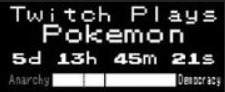
\includegraphics[center]{pictures/AnarchyVSDemocracy.png}
\caption{Anarchy - Democracy voting panel inside the stream}
\end{figure}

\subsection{Communication and context \textit{(or lack thereof)}}

Since \textit{TPP} was playing 24/7, it quickly became difficult to follow the progression of the stream, as one couldn't stay constantly awake and active. The community had to get organized to communicate about the game, strategies, keep tracks of the game progression, even with players all over the globe with different time zones.

\begin{quote}
{\centering"\textit{You cannot pause an online game.}"\par}
\hfill\hfill- Obvious yet recurring internet proverb
\end{quote}

This section aims at listing what actions the twitch community set up in order to tackle the communication problem. First of all, they had to get their hands on a global media that everyone could easily check up on.

\subsubsection{The Chat}

The chat is supposed to be the best vector of communication. It is easy to use, right next to the video stream, and every player has direct access to it, so this was naturally the first idea of what to use in order to reach everyone. Yet, the chat was not really of good use considering that one hundred thousand players at the same time were constantly writing commands to it. It quickly became flooded with commands and thus impossible to read.

What the community came up with are chat filters. Every modern web browser has a console where JavaScript code can be added to any web page. Considering this event was really popular among experienced computer users, some wrote simple to advanced scripts to filter the chat from its commands, quickly evolving into more complex scripts\footnote{Latest version available at https://github.com/jpgohlke/twitch-chat-filter}:

\lstset{language=Java,captionpos=b,breaklines=true,caption={Easy to paste filtering script},label=DescriptiveLabel}
\begin{lstlisting}
(function(){document.body.appendChild(document.createElement('script')).src='http://jpgohlke.github.io/twitch-chat-filter/chat_filter.user.js';})();
\end{lstlisting}

This was a local solution and couldn't be automatically deployed to every player, but it really helped making the chat readable again. With this, people were able to make a normal use of the chat, but this was still not good enough as people were cheering, joking, shouting directions or nonsense. Sometime a link to a reddit discussion managed to sneak through, but the chat was still the battlefield, and strategy is not to be discussed on the battlefield.

\subsubsection{Too many is just enough}
As the chat, even when filtering commands, was flooded with nonsense, the original dedicated way of communicating with everyone was broken. Players then came up with various ways of communicating with each other, quickly setting up :
\begin{itemize}
\item \textbf{A subreddit group :} Reddit.com is a website where anyone can create a category of contents (called subreddit) about anything. In a subreddit, users can create threads of discussion to talk or post pictures. During \textit{TPP}, the subreddit \textit{/r/twitchplayspokemon/} was used as a way to discuss strategies, or post long messages that would not fit in the chat.
\item \textbf{twitchplayspokemon.org :} a dedicated website that launched only a couple days after the game went viral online. The website tracks progression of \textit{TPP} games, and relays other information such as strategies, chat filtering scripts and more.
\item \textbf{A live reddit microblog :} Reddit.com also provides a way to create a microblog. Much like twitter, owner of the microblog can post brief messages. A team of "live redditers" formed around \textit{TPP} in order to provide live information about the game and its state. They had the clever idea to constitute this team with members from several continents, to allow themselves to keep live coverage of the events 24/7. The sun never set on the \textit{TPP} empire.

These live redditers managed to inform the players live on what happened in the stream, but also to link to strategies and try to set goals for the hive-mind to follow. Here are a few examples of the live reddit entries.
\begin{quote}
\textit{- [Strategy] We have options other than to go back to Victory Road. Here is a map detailing alternatives like training AIR Jordan and retrieving TMs.}

\textit{- [Party] 14d13h28m: Air levels up to 25, finally, and learns Body Slam, replacing Sing. The sound of progress.}

\textit{- [Strategy] Here's an updated strategy map for the upcoming Victory Road puzzles! }

\textit{- 15d19h55m Omastar grows to level 46}
\end{quote}
\item \textbf{An IRC channel :}  An IRC channel is a chat much like the Twitch chat. Some players agreed on the use of a chat to communicate and created \textit{Freenode IRC \#TwitchPlaysPokemon} to talk about the game on a less crowded chat.
\item \textbf{A summary on Google doc :} When arriving on the stream, it was easy to grasp the short term goal for the character, like getting into a building, or fighting a Pokemon battle. What was less easy was to grasp a more global state of the game and team. This is why several attempts at tracking the progression of the game, in the form of Google documents, tracking the level and stats of the Pokemons, the location, number of badges, a description of a long term goal and links to the currently adopted strategy (see \textit{Strategies}).

The two mainly used documents are still available at:
  \begin{itemize}
    \item https://sites.google.com/site/twitchplayspokemonstatus/red-archive
    \item http://bit.ly/TPPStatus\_Red
  \end{itemize}
\end{itemize}
These are the main vectors of communication that were available, but possibly hundreds of other arose, as any group of friends playing together might have had their own Facebook group chat as well as their own agenda. This could have gone wrong if everyone was suggesting different strategies, but since ultimately the goal was to beat the game, and since every player knew and remembered how to play \textit{Pokemon : Red}, the multiple sources of information were broadcasting an almost unanimous message. Someone who followed the main medias had a relatively good vision of the progress of the game.

\subsubsection{Strategies}

Strategies, or "strats", is what redditers came up with to try and organize the hive-mind over certain goals. Experienced Pokemon players were thinking in advance on what action would be useful to do in order to ease the game. Then they published sometimes really advanced strategies on reddit, explaining how they would help.

Strategies were written about pretty much everything, short term actions such as "How to beat the ledge" (see \textit{The Ledge}), or on how to defeat a specific enemy. There were also some really detailed and complex schemes, organizing detours to avoid hard parts of the game, or to try and capture a specific pokemon that would facilitate future combats.

The great thing with \textit{TPP} strategies was that they were written while keeping in mind that they were to be adopted by only a part of the hive-mind, in a game were the movements of the players were chaotic on a small scale, and thus reddit strategies were quite different than regular Pokemon strategies. For instance, "detour" strategies were not necessarily made to avoid hard combats, but rather to avoid locations where the movements of the player had to be coordinated. Since the hive-mind was known to randomly toss away objects, strategies involving important objects\footnote{Ex. : http://i.imgur.com/EWVpOKe.png} asked to keep pressing \textit{b} every once in a while to make sure no one opened the menu and tossed the object by accident.

Strategies, once posted, were then suggested via the chat, the IRC channel and the live reddit, discussed, and then accepted or not by the hive-mind.

\subsection{Trolls}

On the internet, a \textit{Troll} is someone who likes to go in the wrong direction, just for the fun of it. That is, starting arguments attacking random strangers on the internet, or flooding off-topic messages. On \textit{TPP}, trolls were trying to sabotage the game. For instance, when the set goal was to enter a building, some people were trying to go to the opposite direction on purpose, just to make the actual players angry. They also set up spambots (see next section).

\begin{figure}[h]
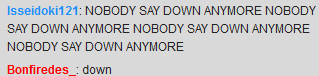
\includegraphics[width=0.5\textwidth,center]{pictures/troll1.png}
\end{figure}

There was a lot of flame regarding trolls during \textit{TPP} because dealing with the chaos was already a hard enough task, dealing with actual human beings trying to break the game on top of that was even harder. Harder because, as someone pointed out, this game was an experiment, and every player was part of it. The original goal was not to beat the game but to see what would happen. Trolls happened, and really nothing could be done about it.

\begin{quote}
\textit{
Nope. No censorship. Bots, trolls and assholes are part of the stream.
The creator stated the idea was to see what happened if the internet played the game. He didn't state it was to see if people on the internet only played the game in a sporting manner. Trolls and bots are part of the internet. The stream consists of the internet. Therefore, bots were part and are part of the stream.}\par
\hfill\hfill- Blizzaldo, Redditer\footnote{Quote from https://www.reddit.com/r/twitchplayspokemon/comments/1ztnct/\#cfx458h}
\end{quote}

\subsection{Spambots}

Spambots, by definition, are bots (scripted programs) that send the same unwanted message, like email ads. It is really easy nowadays to write or find a Twitch Chat Spambot, a program that regularly sends a message to a specific Twitch stream chat.

This is how quickly a lot of bots were sending wrong directions as commands, or even the \textit{start} command, that opens the menu and absorbs the other commands as the character cannot move while in the game menu, and as a \textit{wait} command was introduced later on in democracy mode it gave spambots another way to break the game by making it pause.

Some players also being tech-savvy, they designed scripts meant to analyze the commands given in the chat, just as the game would, but adding statistical analyses to identify spambots. These scripts were then posted through the subreddit\footnote{https://www.reddit.com/r/twitchplayspokemon/comments/1z3e70} to the creator as a suggestion to be implemented, but they were apparently never implemented by the creator.

\subsubsection{Protests}

Spambots are really interesting because they are a way to protest on the internet, they create a flood almost impossible to counter without interrupting the service, like Denial of Service attacks. As bots were not filtered on \textit{TPP}, people protesting to bring back a fully anarchic game set up bots spamming the \textit{anarchy} command, in order to maintain the game in anarchy mode.

An other way of protesting was to flood the commands with the \textit{start9} command, that acted like pressing \textit{start} nine times, opening and closing the game menu several times, effectively breaking the gameplay, even more when the game was in democracy mode, as the number of commands per second was reduced.

\subsubsection{Counter-bots}

In order to fight evil with evil, players also set up spambots, spamming the \textit{b} command, that cancels the currently open menu, thus canceling start bots. The same goes for anarchy / democracy bots.

\subsection{The Ledge}

Sometimes it is the most unexpected problems that stroke. Usually, a normal person can move around in an orderly fashion. But with hundreds of commands at the same time, the character in \textit{TPP} was caught in a whirlwind. This made a lot of small things become great challenges, such as what became known as \textit{The Ledge}\footnote{In \textit{Pokemon} games there are one-way ledges that you jump when going down and can't climb back without coming round.}.

\begin{figure}[h]
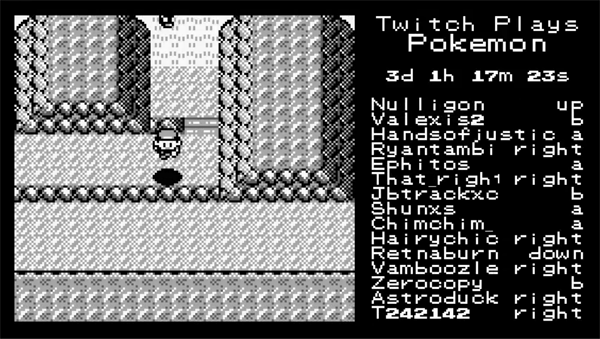
\includegraphics[width=0.5\textwidth,center]{pictures/ledge1.png}
\end{figure}

The first problematic ledge is in the town of Viridian City, long before the democracy mode was implemented, where in order to enter a mandatory building the player has to execute a specific sequence of commands, going down toward a ledge and then turning left for a series of moves until finally reaching a building. During the left series, there is no gap between the character and the ledge, meaning that any down command will result in a fail and players have to start over.
It took the community nine hours to beat this ledge. The reason was that when the character reached the top of the town and had to go down, hundreds of players inputted \textit{down} at the same time, thus when it was time to turn left, the character was still executing \textit{down} commands, and that is not accounting for spambots.

\begin{figure}[h]

\includegraphics[width=0.5\textwidth,center]{pictures/ledge2.png}
\end{figure}

One redditer (a member of the subreddit community) eventually came up with a strategy\footnotetext{https://www.reddit.com/r/twitchplayspokemon/comments/1y1ee8/} and succeeded in getting it adopted by the community, by also posting it on the IRC channel and other social media. One player posted it to Mibbit, an other IRC webchat, and got five hundred users to adopt the strategy in bulk. Combined with other efforts to get the strategy adopted by the hive-mind, this was enough to win this puzzle.

The goal of the strategy was to use the \textit{start} command, which opens the game menu. While in the game menu, the character cannot move, thus the down commands would have no effect on the character. Once the flood of down commands passed, the same pattern is repeated with left and up into the building.

The strategy was successful, but as one can imagine, this is not the only ledge in the \textit{Pokemon : Red} game. The democracy mode introduced later on sometimes was activated during ledge puzzles, helping to get through. In the following of the game and in the next games of \textit{TPP}, this lead to people doing analyses\footnote{https://www.reddit.com/r/twitchplayspokemon/comments/25vtkv/} of upcoming ledges beforehand, in order to prepare for them:

\begin{quote}
[\dots] \textit{there's fortunately a rock just before the ledge which will "eat" some extra down inputs. This down-oriented ledge is a 8x2-tile, plus a rock climb at the 6th tile of the ledge that we must do. So there can be too many right inputs, we will need some left and up inputs as well.}\par
\hfill\hfill- toto2379, Redditer
\end{quote}

\section{Motivation}

\textit{TPP} was hard. It was a struggle to play it until the last moment, even with all the organization. Some players sacrificed time and sleep to try and coordinate the hive-mind. Most of the media used for \textit{TPP} (google docs, reddit) are free to use, but others are not, for instance setting up a hosting solution for twitchplayspokemon.org is not free. People were then spending time and money, much like volunteer work, on helping other people in a game that remains purely virtual. This is a recurring pattern on the internet and video games, people putting a lot of effort into something that won't bring back anything other than a rewarding feeling of achievement.

\begin{figure}[h]
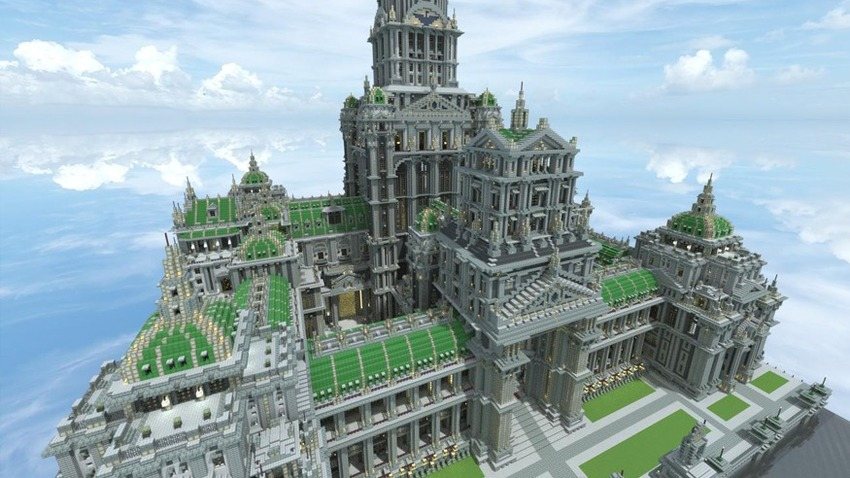
\includegraphics[width=0.6\textwidth,center]{pictures/Minecraft.jpg}
\caption{A gigantic palace built in minecraft}
\end{figure}

People on the internet like a challenge. \textit{TPP} was a great challenge, as it brought together countless gamers who spent their childhood playing \textit{Pokemon}. The motivation of the community was also based on the novelty of the concept, and the reward of being part of a great \textit{Pokemon} adventure that felt impossible.

Players from all around the world agreed that \textit{TPP} was a big moment in video game history, and worked hard to achieve it.
\begin{quote}
\textit{
I wish people got this involved in actual politics, ie: gerrymandering, bribery, election fraud, etc.
}\par
\hfill\hfill- pseudolobster, Redditer
\end{quote}

\newpage

\section{Follow-up}

The success of uniting people around what is considered to be \textit{the biggest "we" moment in video game history} still amazes today.
In the end, the \textit{TPP} community proved to be quite thorough in setting up a functioning ecosystem that takes into account the fact that tens of thousands of users were playing simultaneously, and the proportion of chaos involved.

In the end, the players who took charge of the organization of Twitch didn't have much choice but to set up elsewhere than on Twitch since the platform didn't have other vectors of communication than the chat. People had to settle elsewhere and naturally chose well-known, accessible, free platforms like Google Docs or Reddit.

The \textit{Twitch Plays Pokemon} channel lives on to this day, having played the following \textit{Pokemon} titles. The newer the game the harder, but the stream also lost almost all its popularity and it is now easier to organize the crowd. Like any viral internet event, \textit{TPP} lead to various products like merchandise, sweaters and T-shirts, but also other video games on Twitch, such as \textit{Twitch Plays Zelda}, \textit{Twitch Plays Tetris}, and more surprising concepts like \textit{Fish Plays Pokemon}, a Twitch stream where a fish tank is filmed, and the fish triggers commands upon entering certain zones of the fish tank. Needless to say, the fish didn't go very far in the game, but still further than \textit{Potato Plays Pokemon}, where the same concept was applied to a potato on a plate. This stream is still stuck on the \textit{New Game} screen.

\begin{figure}[h]
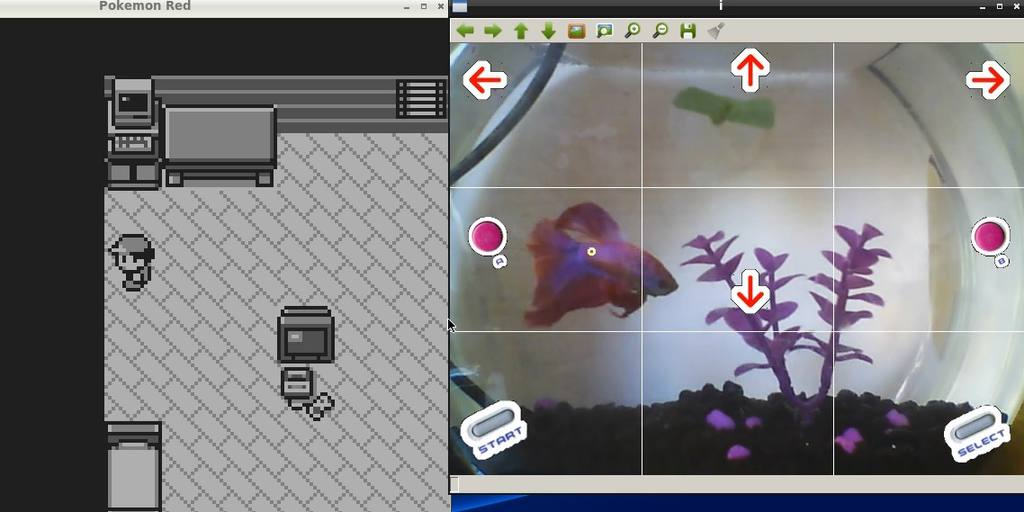
\includegraphics[width=0.6\textwidth,center]{pictures/FishPP.jpg}
\caption{\textit{Fish Plays Pokemon}}
\end{figure}

\end{document}